%% IMPORTANT! COMPILE WITH -shell-escape option for ffcode to work

\documentclass[a4paper,11pt]{article}
% Useful packages
\usepackage{amsmath}
\usepackage{amssymb}
\usepackage[utf8]{inputenc}
\usepackage[pdftex]{graphicx}
\usepackage{etoolbox}
\usepackage[svgnames]{xcolor}
\usepackage{tcolorbox}
\usepackage{fancyhdr}
\usepackage{matlab-prettifier}
\usepackage{enumerate}
\usepackage[shortlabels]{enumitem}
\usepackage{amsthm}
\usepackage{ffcode}


% Page size
\textwidth=170mm
\oddsidemargin=0mm
\evensidemargin=\oddsidemargin
\textheight=230mm
\topmargin=-10mm

%Section numbering
\setcounter{secnumdepth}{-1}
%opening
\title{EITF75: Lab /number/ Report}
\author{Student 1 name and Student 2 name}
\begin{document}

\raggedright
\maketitle
Include all your solutions to the Preparation exercises and document your Lab 
tasks. Use the red 'Include in lab report:' boxes in the lab instructions to make 
sure you do not forget anything.
\section{Preparation exercises}
\subsection{Problem 1}
\subsubsection{a}

We know that F is 4 times smaller than Fs and we then calculate the equation below. 
\[
\omega_{0} = 2 \pi \frac{F_{0}}{F_{s}} 
\]
Resulting in
\[
\omega_{0} = \frac{\pi}{2}
\]
We also know that the zeroes comes in pair which mean we also have one at 
\[
\omega_{0} = -\frac{\pi}{2}.
\]
This means we have our zeroes along the y-axis and they can be written as
\[
(1-e^{j\frac{\pi}{2}}z^{-1})(1-e^{-j\frac{\pi}{2}}z^{-1})
\]
This gives us
\[
H_{1}(z) = \frac{(z-e^{j\frac{\pi}{2}})(z-e^{-j\frac{\pi}{2}})}{z^2} = \frac{z^2-2zCos(\frac{\pi}{2})+e^{j(\frac{\pi}{2}-\frac{\pi}{2})}}{z^2} = \frac{z^2+1}{z^2}.
\]
The last thing needed is to substitute 
\[
z = e^{j2\pi f} 
\]
Inserting this with f = 1/2 should give us 
\[
H_{1}(f) = 1 =  b_0\frac{e^{j\pi}^2 + 1}{e^{j\pi}^2} = 2b_0 \xrightarrow{} b_0 = \frac{1}{2}
\]
\subsubsection{b}
%plot pole zero av filtret
\subsubsection{c}
%plot mag o fas filtret. 0<f<0.5
\[
H_{2}(f) = 1 =  b_0\frac{e^{j\pi}^2 + 1}{e^{j\pi}^2 + 0.95^2} \xrightarrow{} b_0 = 0.95125
\]
\subsubsection{b}
%plot pole zero av filtret
\subsubsection{c}
%plot mag o fas filtret. 0<f<0.5
Our filter is now more accurate on the frequency that we want to remove. Before we have a dampening effect on more than the area we want to dampen. 
%Kolla skillnaden i fas graferna också. 

\subsection{Problem 3}
\subsubsection{a}
\[
y(n) = x(n) + \alpha x(n-D)
\]
Which gives us
\[
h(n) = \delta(n) + \alpha\delta(n-D)
\]
\subsubsection{b}
%plot magnitude och pole zero 
\subsubsection{c}
\[
H(\omega)^{-1} = \frac{1}{1 + \alpha e^{-jwD}}
\]
Now going to the Z-transform of this we get.
\[
\frac{z^D}{z^D + \alpha}
\]
Which means we get D zeroes at Z = 0. And the poles at
\[
poles = \sqrt[D]{-\alpha}
\]
\subsubsection{d}
%plot magnitude och pole zero, kolla skillnad. 
\subsubsection{e}
As long as 
\[
|\alpha| < 1
\]

\section{Laboratory tasks}

\subsection{Lab Task 1}
To playback the audio files as instructed in lab task 1, we used the following MATLAB code:
%This environment shows how to get 'nice' presentation of MATLAB code in LaTex:
\begin{ffcode} 
%% Task 1
%Read HQmusic.wav from file (y = signal, f = sampling freq.)
[y, f] = audioread('MATLAB_FILES/HQmusic.wav');
%Playback HQmusic.wav at reconstruction freq. f_pb (Change f_pb according
%to task)
f_pb = f / 2;
soundsc(y, f);
\end{ffcode}

It was noted that changing the reconstruction frequency ("f\_pb" in code) to half of the sampling frequency ($\frac{F_s}{2}$) both lowered the volume and made the pitch sound lower. Changing f\_pb to $2F_s$ had the opposite effect on the pitch.
\subsection{Lab Task 2}
The signal yielded from task 1 was plotted, both in the time and frequency domain. Time domain signal can be seen in figure 1 and the frequency domain signal can be seen in figure 2.

\begin{ffcode} 
%% Task 2
%plot time domain signal
secs = length(y) / f;
time = linspace(0, secs, length(y));
plot(time, y)
hold on
%plot freq. domain signal
Spectrum_PLOT(y, f);
\end{ffcode}

\begin{figure}[H]
    \centering
    \hspace{-40pt}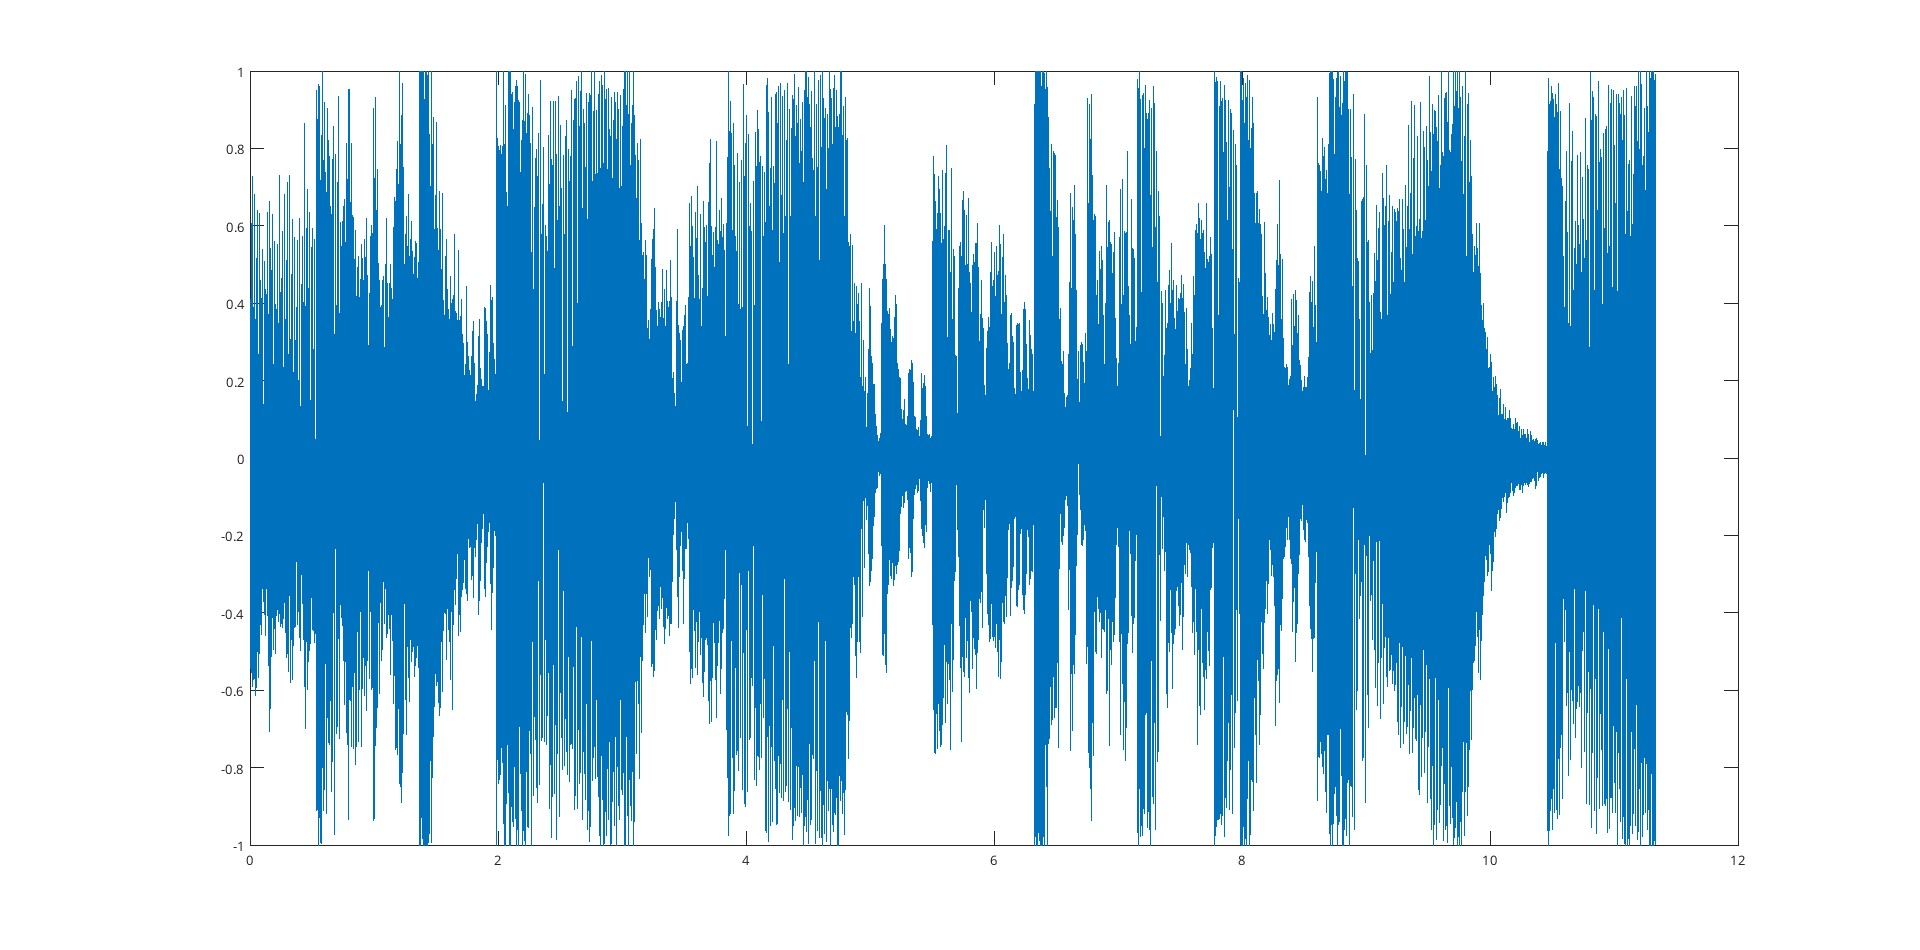
\includegraphics[scale = 0.2]{./images/Task2-PSD.jpg}
    \caption{Time domain plot of HQmusic.wav's signal}
    \label{fig:Task 2 Time domain}
\end{figure}

\begin{figure}[H]
    \centering
    \hspace{-60pt}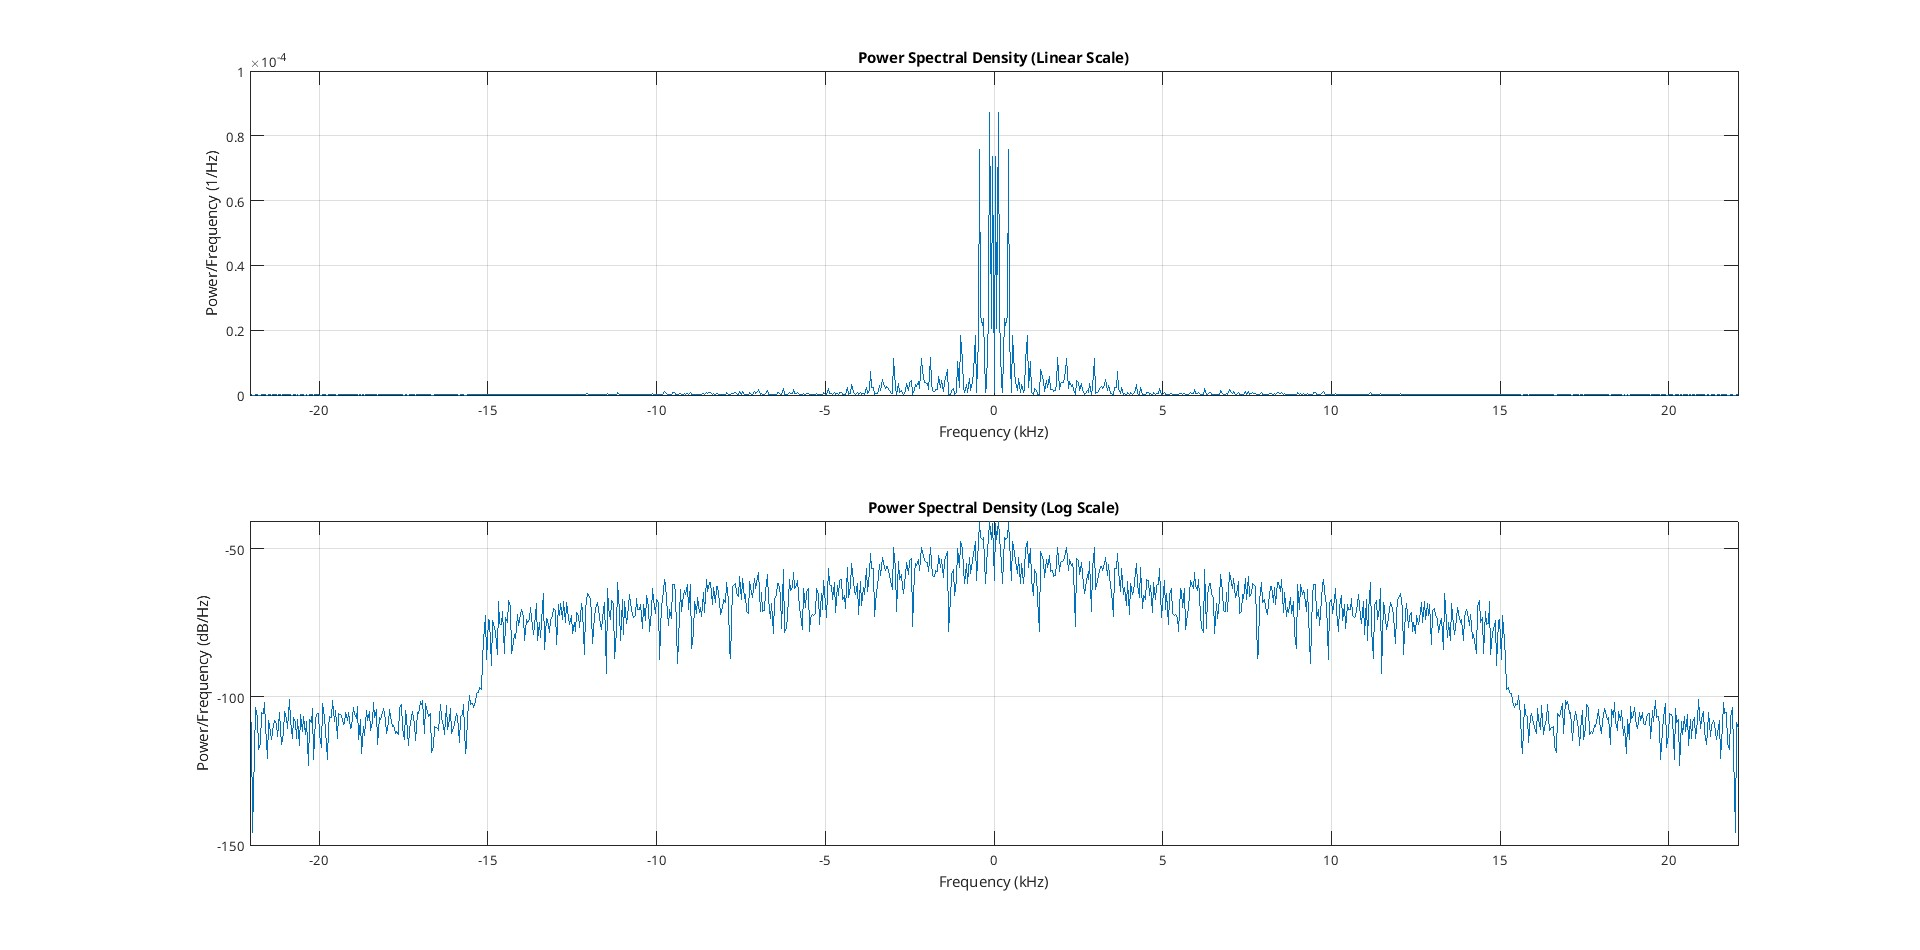
\includegraphics[scale = 0.28]{./images/Task2-FFT.jpg}
    \caption{Frequency domain plot of HQmusic.wav's signal}
    \label{fig:Task 2 Freq. domain}
\end{figure}


As can be seen in figure 2, the most prominent (largest) frequency component was 120 Hz. Since the audio was bass-heavy music, this is a reasonable result.

\subsection{Lab Task 3}
For task 3, a simple moving-average filter was applied to HQmusic.wav's signal. The following MATLAB code was used to apply the filter:

\begin{ffcode}
%% Task 3
filter = 1/5*ones(5,1);
%discard first 4 samples of output
u = conv(y, filter);
u = u(5:end);
soundsc(u, f)
Spectrum_PLOT(u, f)
\end{ffcode}

The filtered signal can be seen in figure 3.
\begin{figure}[H]
    \centering
    \hspace{-60pt}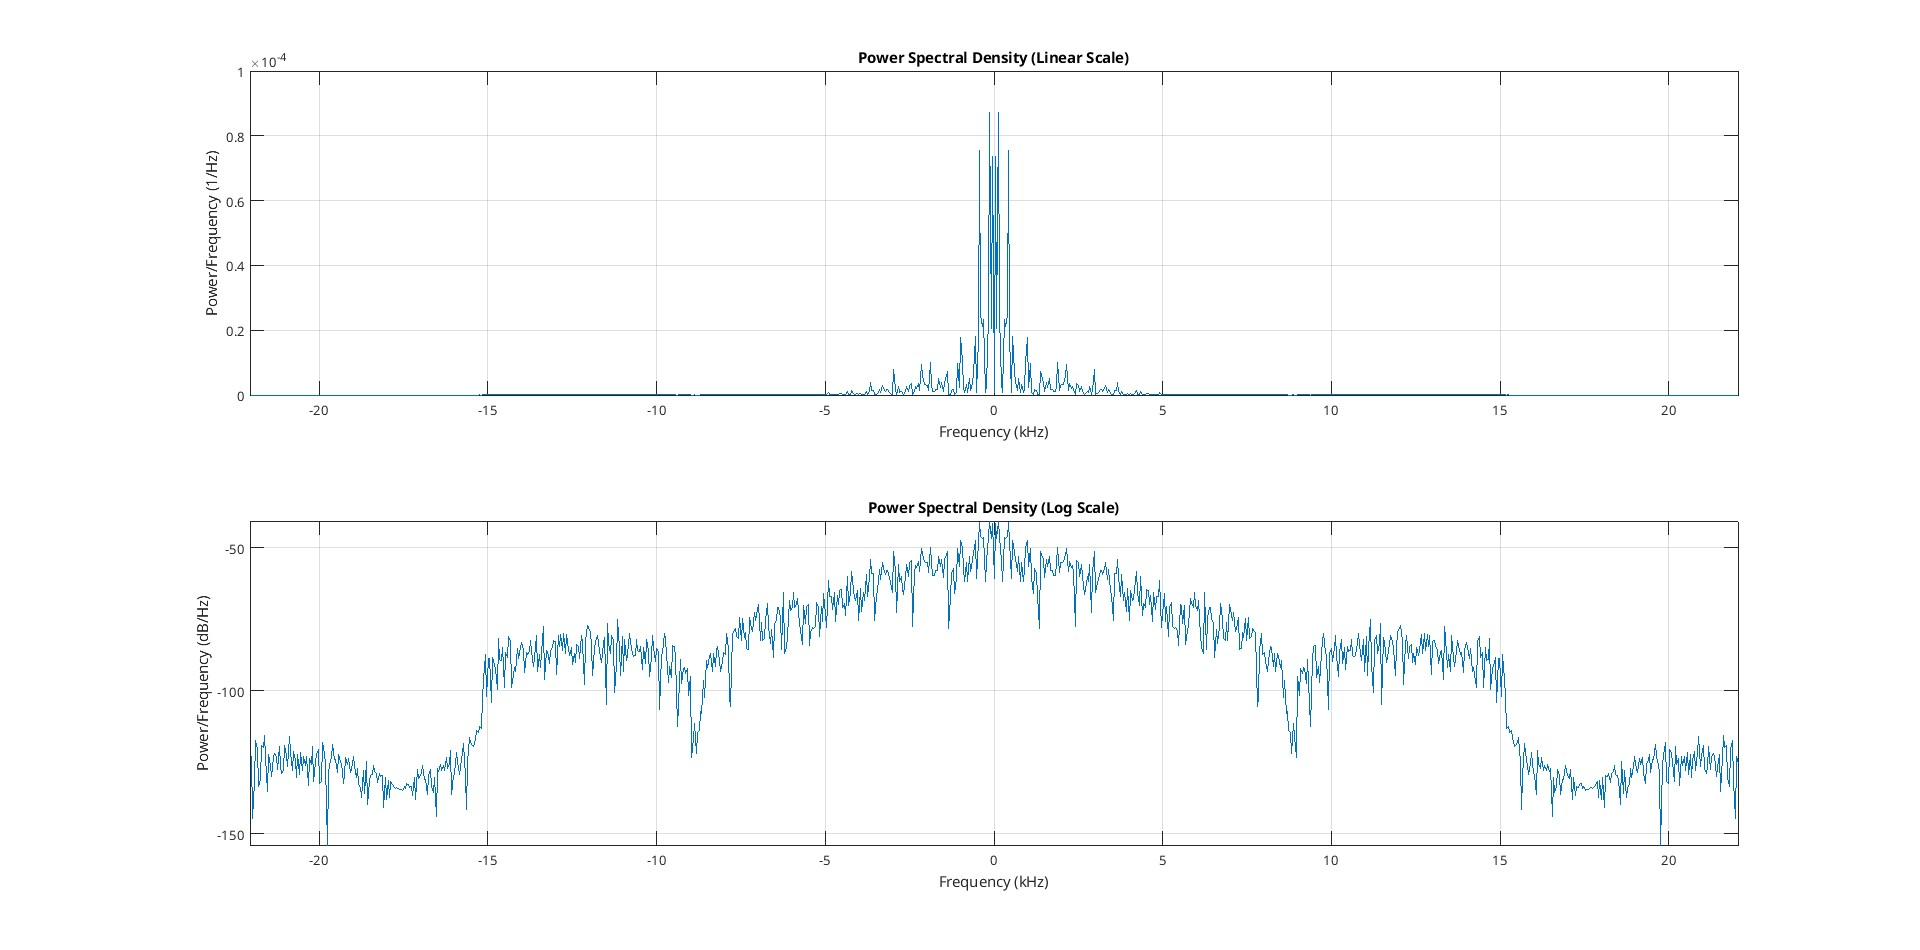
\includegraphics[scale = 0.28]{./images/Task3-filtered.jpg}
    \caption{Frequency domain plot of HQmusic.wav's signal, with a moving average filter applied}
    \label{fig:my_label}
\end{figure}
This filter removed more of the signals higher frequencies (treble). This is due to the filter taking the average amplitude of frequencies over 5 samples. Since higher frequencies are less prominent in the audio (as seen in figure 2), these frequencies are filtered. Increasing the length from 5 to 15 amplified this effect. Removing even more of the higher signals, leaving mostly bass.

Differences between the linear plots before and after the filter are minimal. The log-plotted figures, however, have notable dips around 8.9 kHz. The valleys starting at 15 kHz have a more rounded appearance after the filter.
\subsection{Lab Task 4}
For task 4 white noise was added using 
\begin{ffcode}
%% Task 4
% add noise
y_noisy = y + 0.1*randn(length(y), 1);
%soundsc(y_noisy, f)
Spectrum_PLOT(y_noisy, f)
\end{ffcode}
in MATLAB. The signal with added noise can be seen in figure 4.
\begin{figure}[H]
    \hspace{-55pt}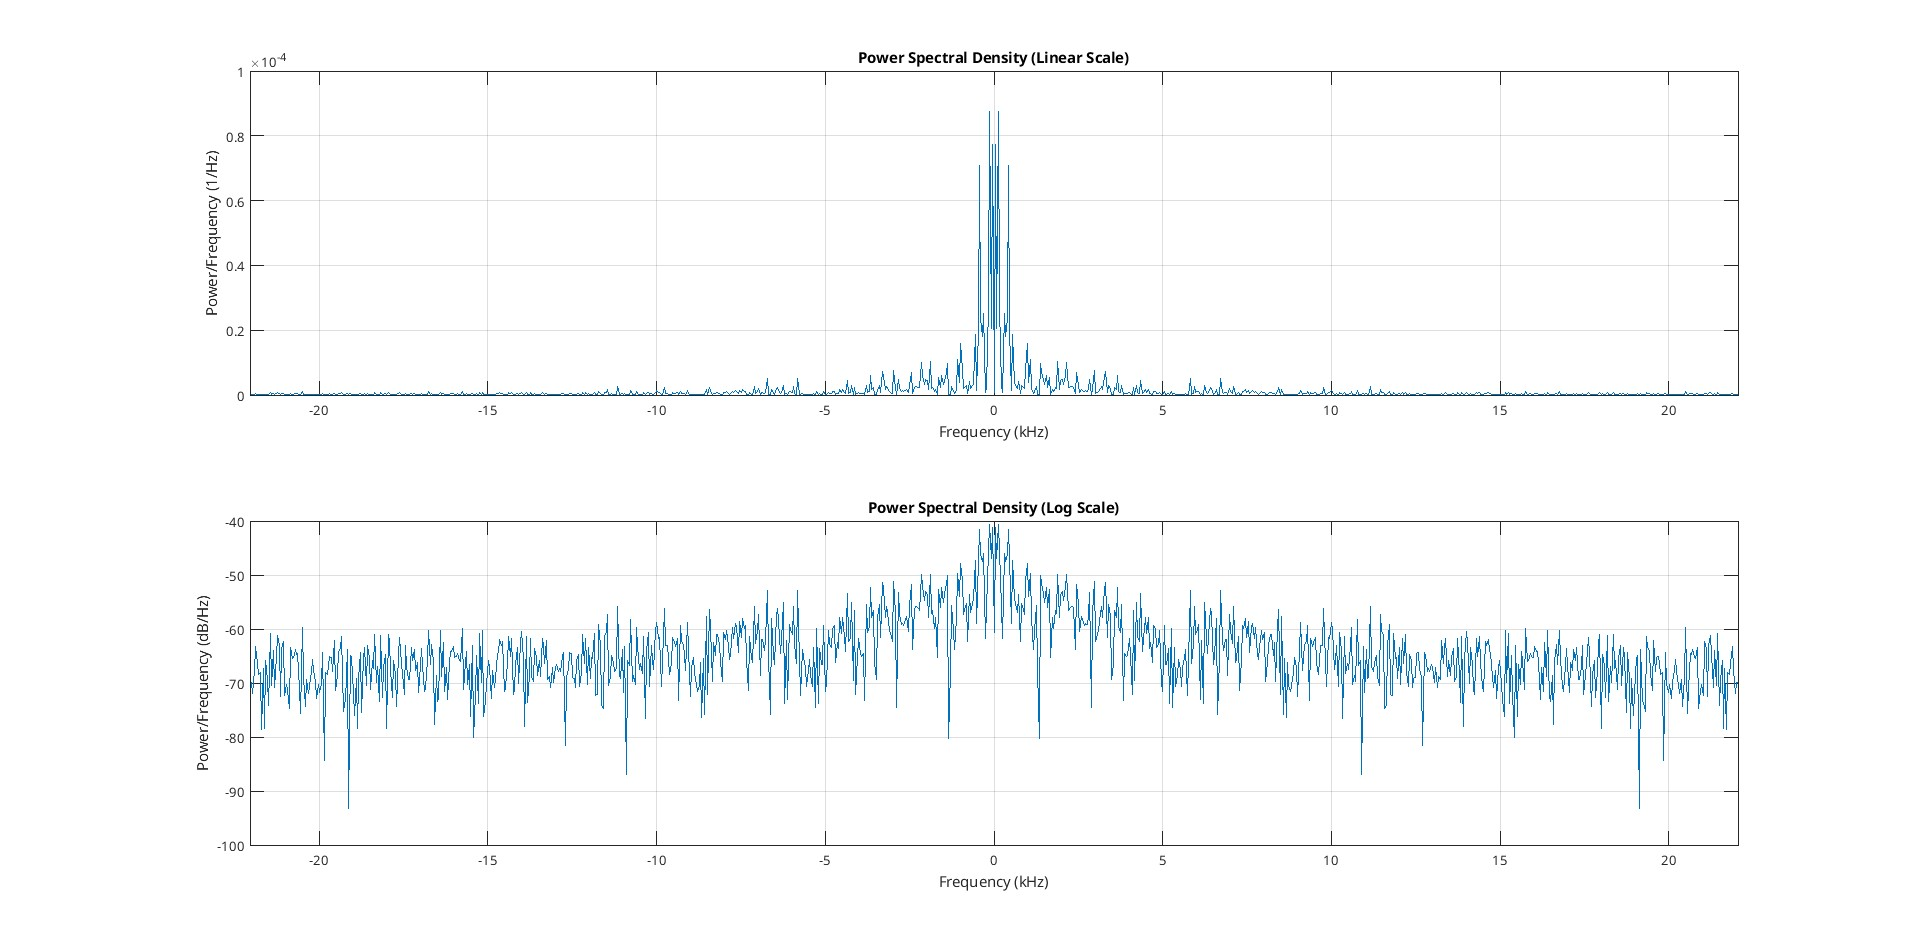
\includegraphics[scale=0.28]{./images/Task4-noisy.jpg}
    \caption{HQmusic.wav's signal with an added Gaussian white noise}
    \label{fig:my_label}
\end{figure}

Afterwards, the noise was filtered by passing the noisy signal through a moving average filter.
\begin{ffcode}
% filter noise
filter = 1/5 * ones(5,1);
u_noisy = conv(y_noisy, filter);
u_noisy = u_noisy(5:end);
soundsc(u_noisy, f)
Spectrum_PLOT(u_noisy, f)
\end{ffcode}
The plot of the filtered signal can be seen in figure 5
\begin{figure}[H]
    \hspace{-40pt}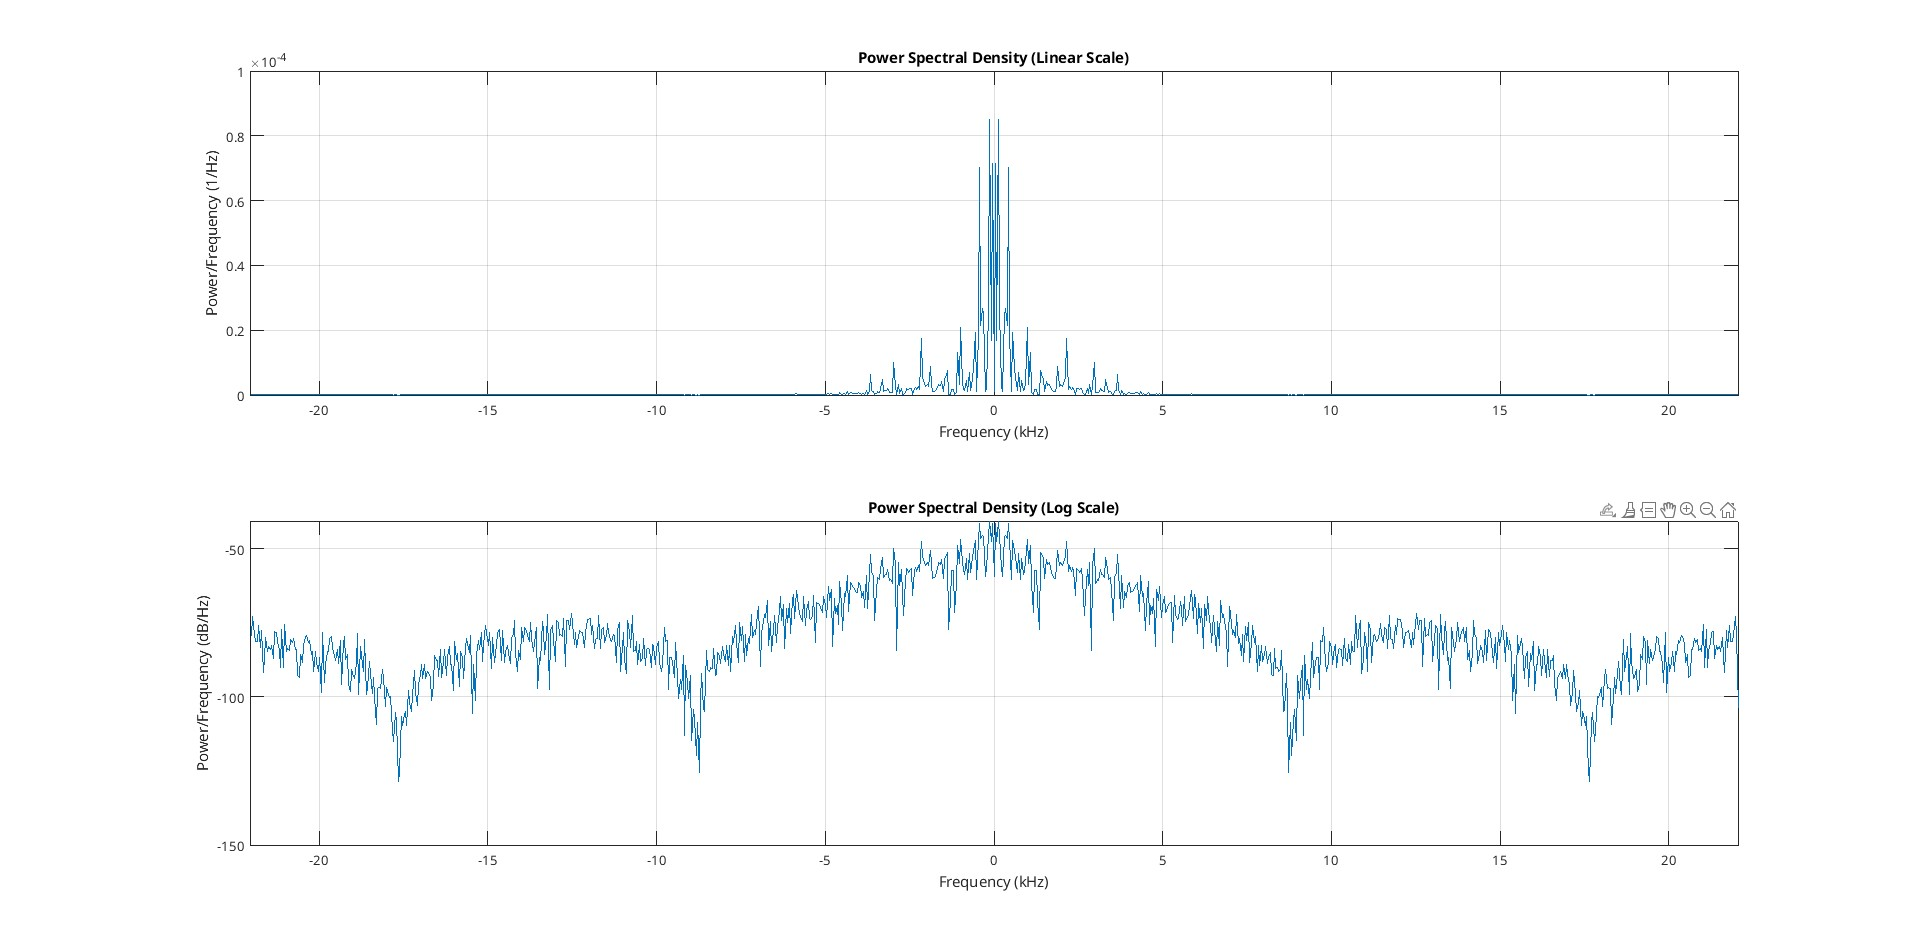
\includegraphics[scale=0.28]{./images/Task4-filtered}
    \caption{Signal from figure 4, passed through a moving average filter of length 5}
    \label{fig:my_label}
\end{figure}
% Nollställen i n*fs / 5 pga faltning med 1/5
As can be seen, the filter reduced the amplitude of the noise considerably (though it did not completely remove the noise), however some sharp dips can be seen around multiples of $\frac{1}{5} \cdot F_s$
\subsection{Lab Task 5}
\begin{figure}[H]
    \centering
    \includegraphics[scale=0.4]{./images/pole-center.png}
    \includegraphics[scale=0.4]{./images/pole-zero.png}

    \caption{Side by side comparison of IIR-filter with poles in origin (left) and poles near zeroes (right)}
    \label{fig:my_label}
\end{figure}
Skriv nåt om polplacering
\begin{figure}[H]
    \centering
    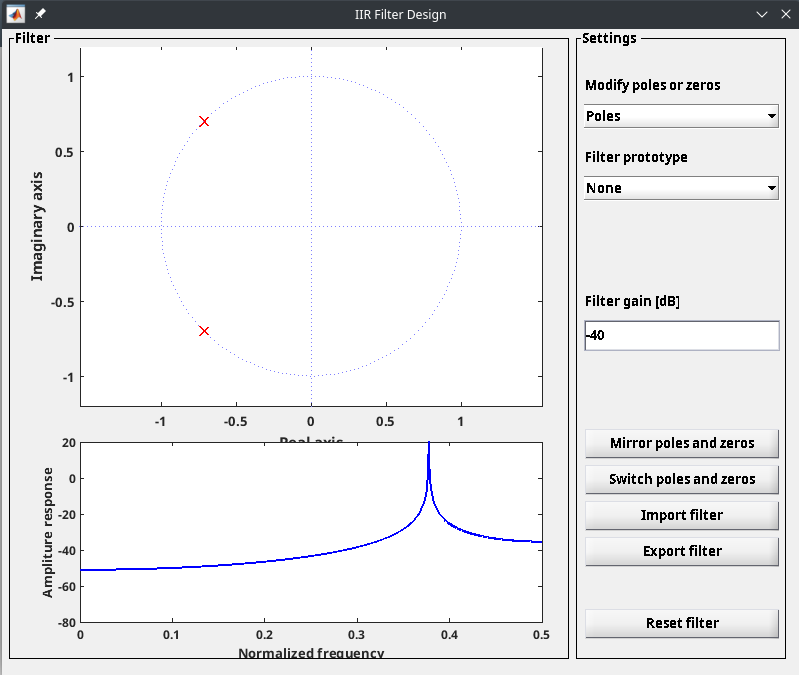
\includegraphics[scale=0.6]{./images/2ndorder-pole.png}
    \caption{Second order pole placed on the unit circle}
    \label{fig:my_label}
\end{figure}
Skriv nåt om polerna + något om pol från $\omega = 0$ till $\omega = \pi$
\subsection{Lab Task 6}
For task 6, the the same audio file used in previous tasks ('HQmusic.wav') was used. A sinusoid distortion was added in MATLAB. Figure 8 contains the power spectral density-plot of the distorted signal.
\begin{figure}[H]
    \hspace{-50pt}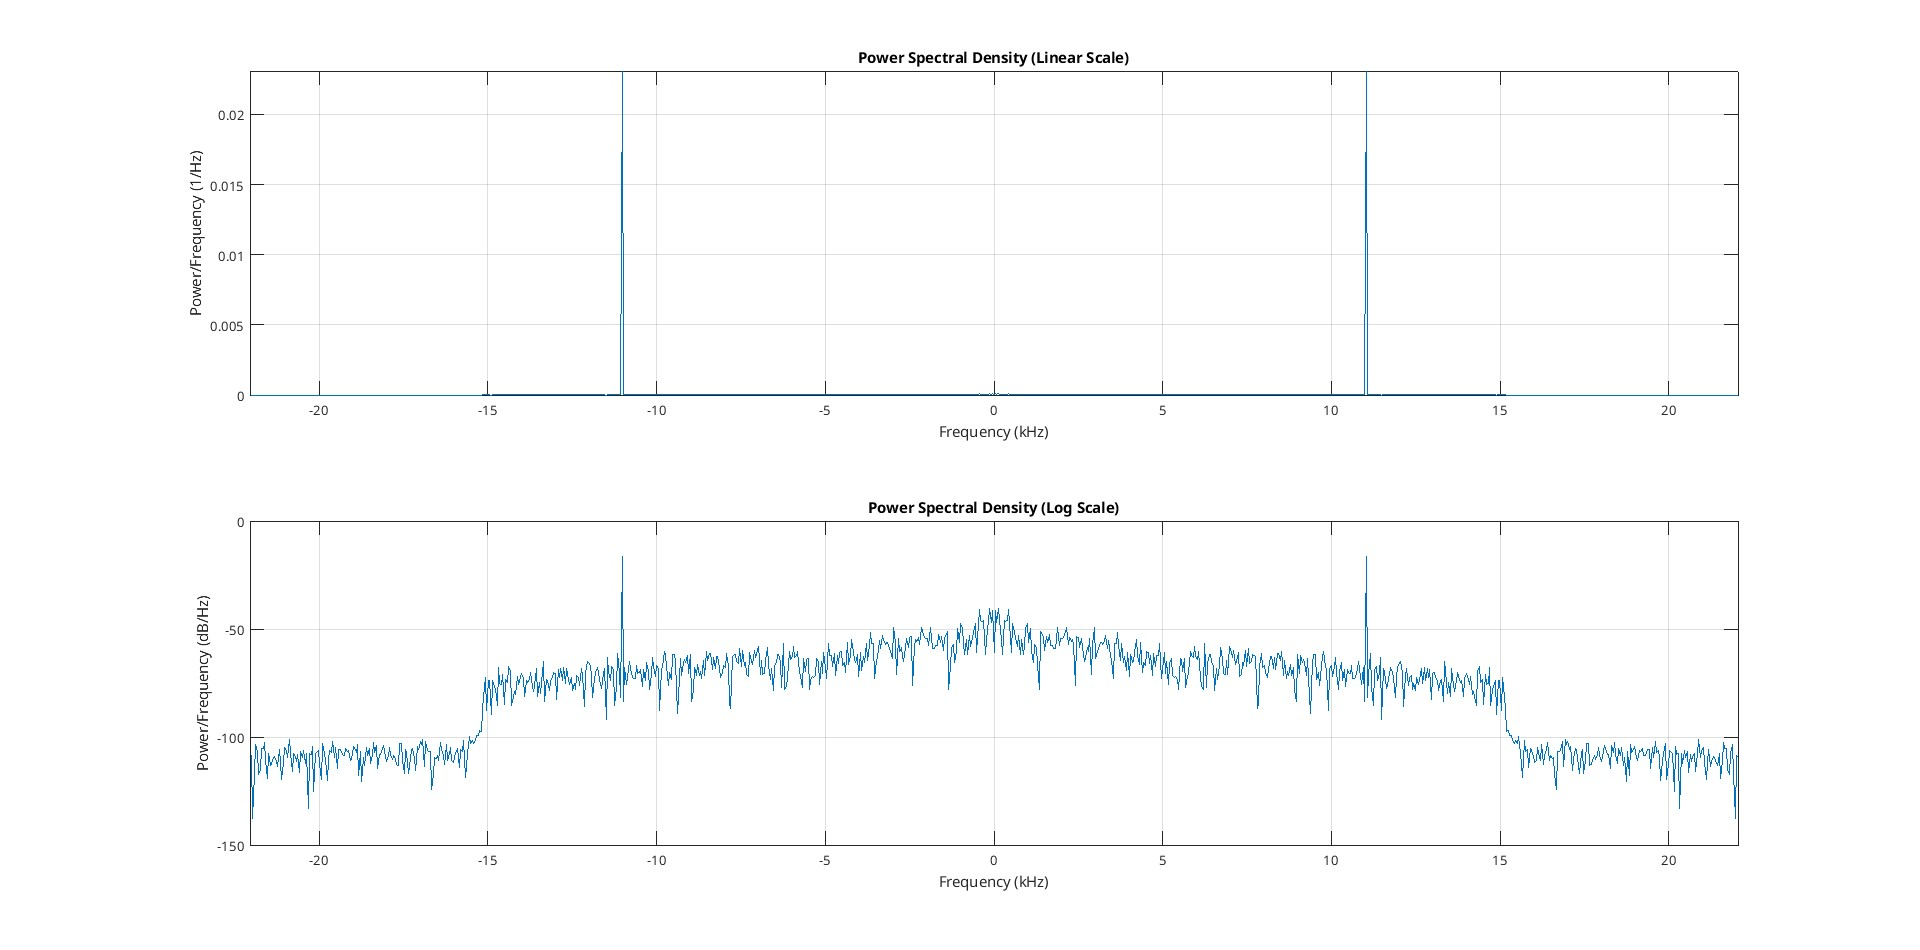
\includegraphics[scale=0.28]{./images/Task6-FFT.jpg}
    \caption{Frequency domain plot of the distorted signal created in task 6}
    \label{fig:my_label}
\end{figure}
\subsection{Lab Task 7}
\subsection{Lab Task 8}
\subsection{Lab Task 9}
\subsection{Lab Task 10}
\subsection{Lab Task 11}
\end{document}